%*****************************************************************
\subsection{Calibration Results}\label{sub:bc_calibration_results}
%*****************************************************************

% Introductory Paragraph
After discarding the samples from the initial burn-in periods,
the remaining posterior samples can be analyzed to investigate the constraining power of the data (as well as the chosen schemes) and the possible correlation structure of the parameters.
The posterior samples of the calibration with model bias term is mainly presented, while the graphical representation of the posterior samples from the other calibration schemes can be found in Appendix~\ref{app:mcmc_samples}.

% Explaining corner plot
The results of calibrating the $8$-parameter model with model bias term is presented in a corner plot shown in Fig.~\ref{fig:ch5_plot_ens_all_disc_centered}.
\marginpar{Corner plot}
A corner plot \cite{Foreman-Mackey2016} depicts the univariate ($1$-dimensional) and the bivariate ($2$-dimen\-sional) marginals of the posterior samples and it provides information on the possible correlation structures between pairs of model parameters.
That is, it projects the multi-dimensional posterior distribution into each of the $1$-dimensional and $2$-dimensional subspaces (see the illustration for Gaussian marginals in Chapter~\ref{ch:gp_metamodel}).

% Diagonal Elements
The univariate marginals are shown as the diagonal elements of the plot.
\marginpar{Corner plot, diagonal element, univariate marginal}
In the diagonal elements of Fig.~\ref{fig:ch5_plot_ens_all_disc_centered}, solid lines indicate the $95\%$ \glspl[hyper=false]{hpdi} \cite{Hyndman1996} computed from the univariate samples, while dashed and dotted lines indicate nominal parameter values and posterior median parameter values, respectively.
Note that the range for each of the model parameters in the plot corresponds to the respective prior uncertainty range.

% Off-diagonal elements
The bivariate marginals of the posterior distribution are shown as the off-diagonal elements of the plot.
\marginpar{Corner plot, off-diagonal element, bivariate marginal}
Because correlation is symmetric, only the lower half portion of the plot is shown.
In this adaption of corner plot, hexagonal binning \cite{Carr2015} is used to provide the ($2$-dimensional) data aggregation method to deal with the large number of posterior samples.
In the off-diagonal elements of Fig.~\ref{fig:ch5_plot_ens_all_disc_centered}, lighter color shading (i.e., more intense color) indicates the region of the parameter space that is denser with sampled points.
The correlation between each pairs of parameters can be preliminary inferred from the shape of the bivariate marginals while the exact number for the color scale is unimportant.

% Explaining the figure, univariate marginal
In Fig.~\ref{fig:ch5_plot_ens_all_disc_centered}, the most constrained parameters (from either side of the prior range) are the \texttt{iafbIntDr}, \texttt{dffbIntDr}, \texttt{dffbVIHT}, \texttt{dffbWHT}.
Some parameters are mostly constrained in one side (most notably \texttt{gridHT}), while \texttt{tQuench} is the least constrained by the data and the calibration scheme.

\begin{sidewaysfigure}
	\centering
	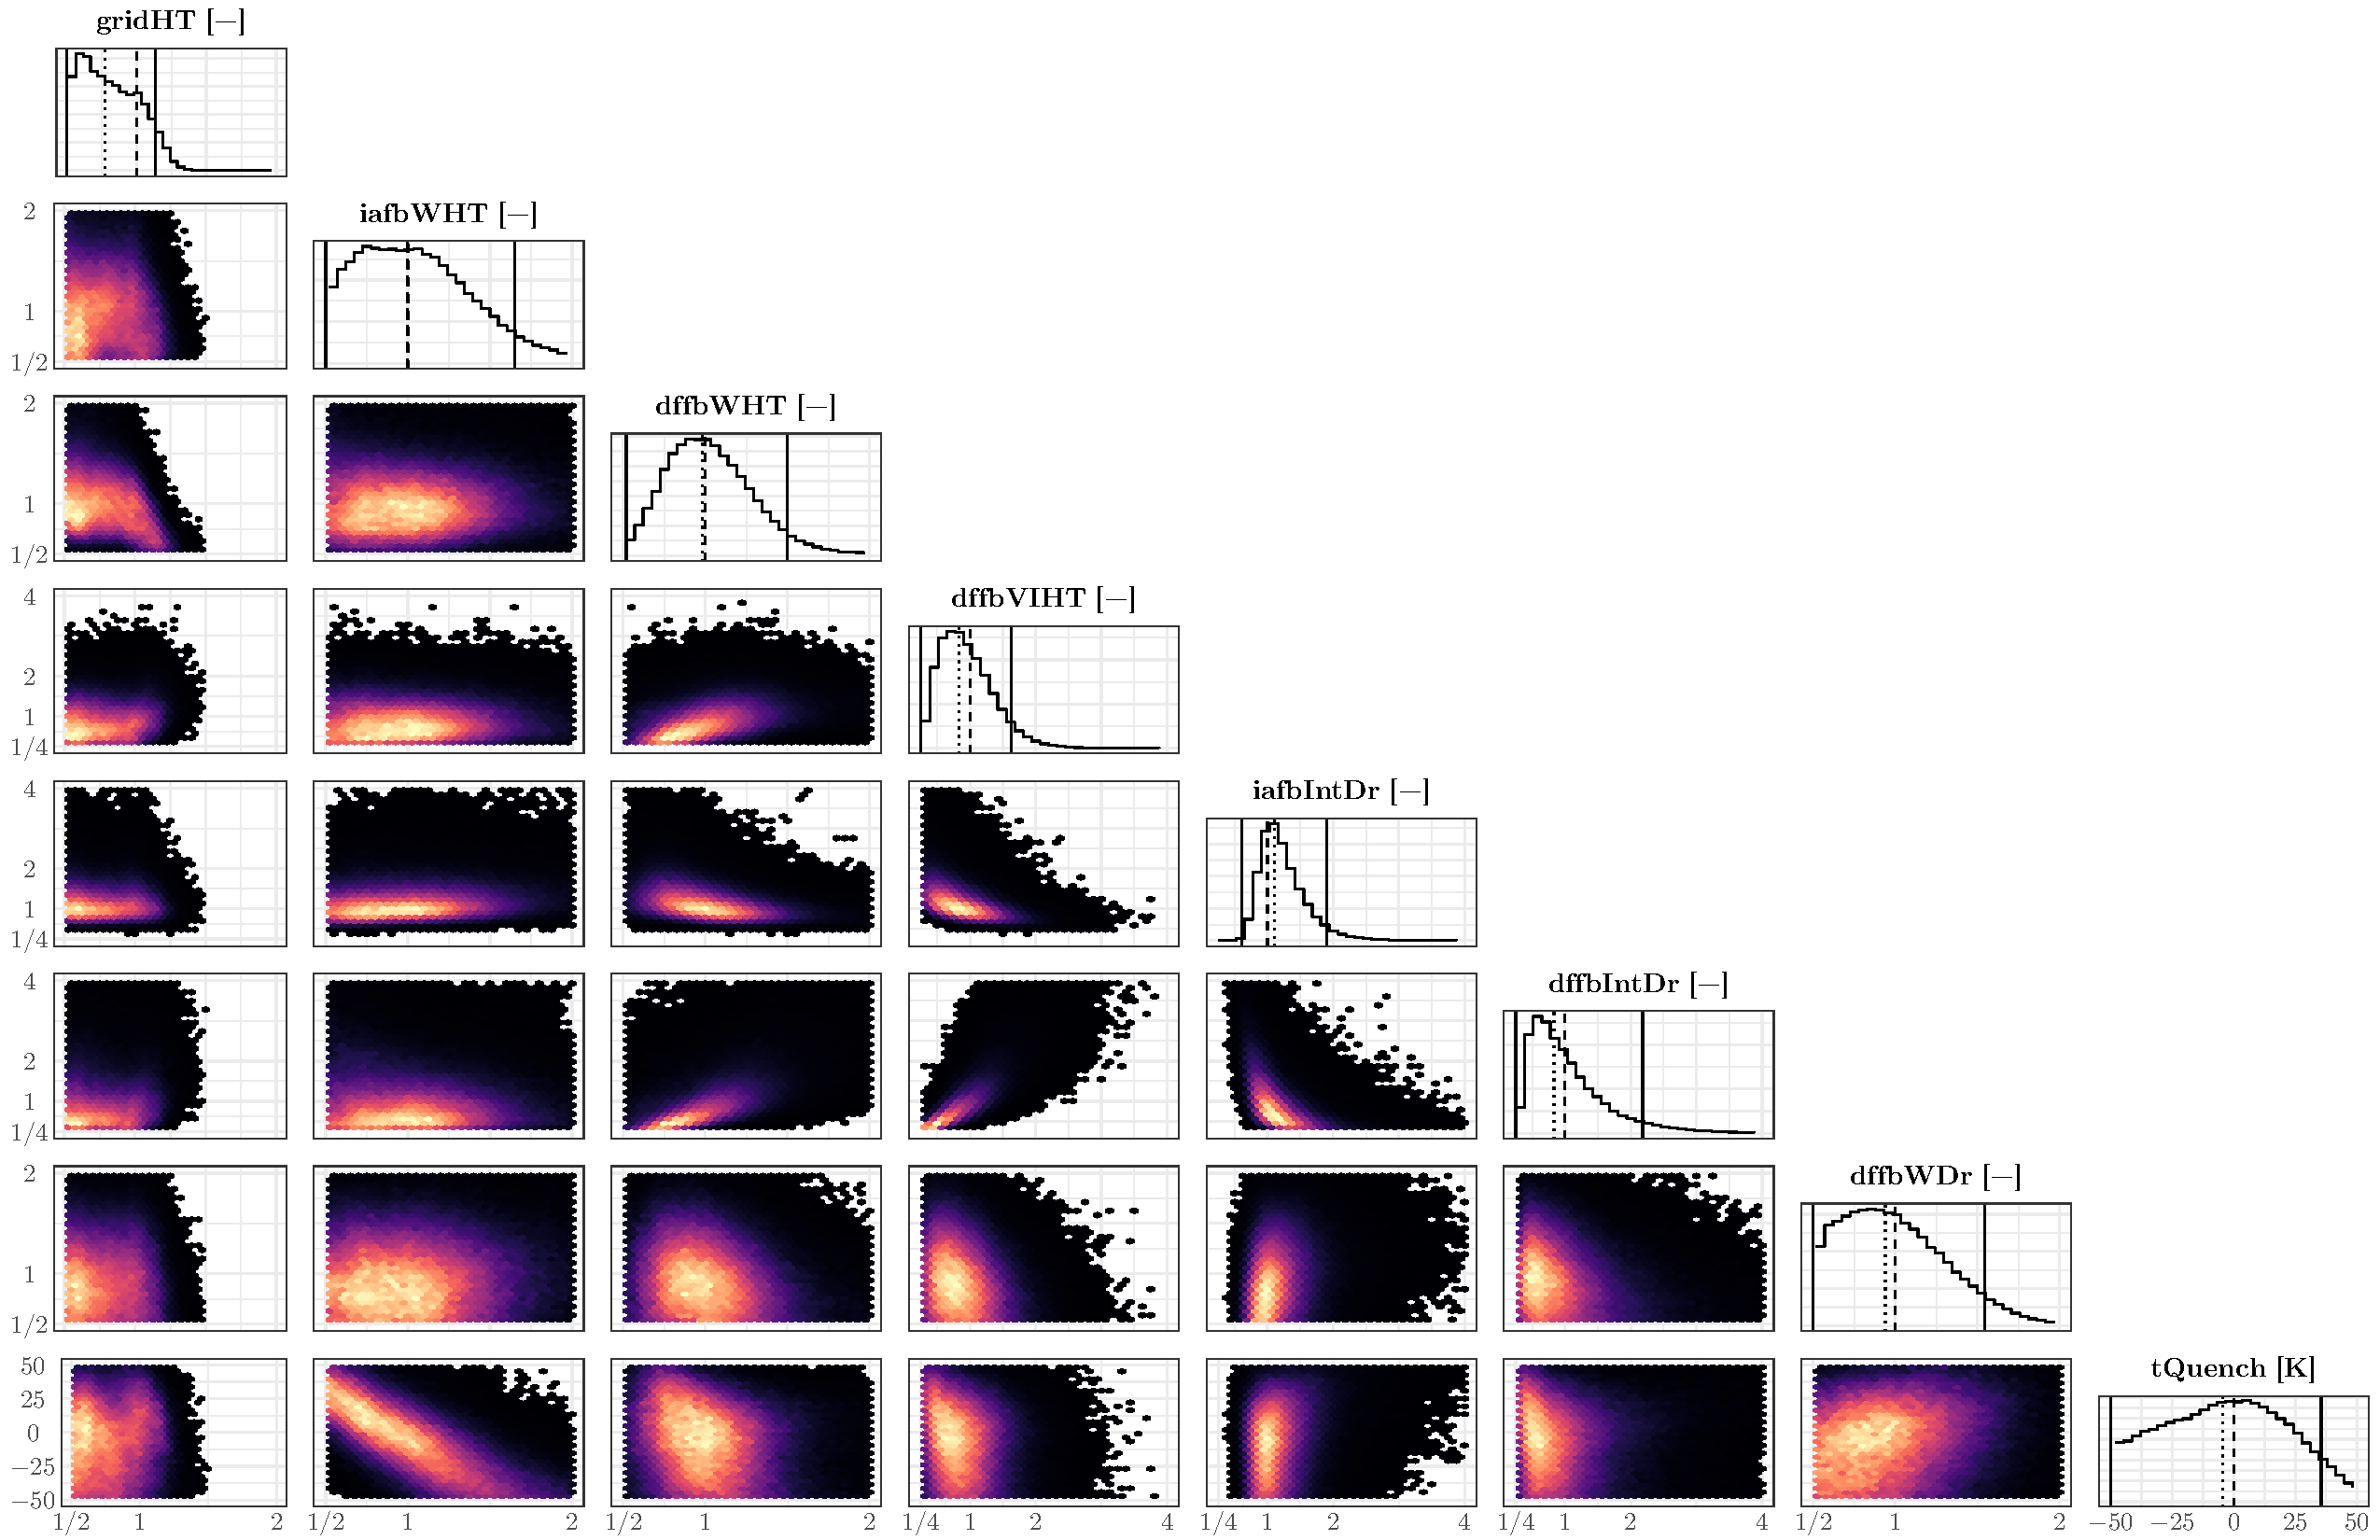
\includegraphics[width=0.90\textwidth]{../figures/chapter5/figures/plotEnsAllDiscCentered}
		\captionof{figure}[Univariate and bivariate marginals of the posterior samples for each of the $8$ model parameters. Calibration with model bias term.]{Univariate and bivariate marginals of the posterior samples for each of the $8$ model parameters. Solid lines, dashed, and dotted lines indicate the \glspl[hyper=false]{hpdi}, the nominal parameter values, and the posterior median parameter values. Calibration with model bias term.}
	\label{fig:ch5_plot_ens_all_disc_centered}
\end{sidewaysfigure}

% Explaining the figure, bivariate marginal
The figure also depicts the correlation structures between pairs of model parameters.
In that case, the values of a model parameter that is consistent with the experimental data depends on the values of another parameter. 
Although most pairs are largely uncorrelated, the parameter \texttt{dffbIntDr} is strongly correlated with \texttt{dffbWHT}, \texttt{dffbVIHT}, and \texttt{iafbIntDr}.
The parameter \texttt{iafbWHT} is also correlated with \texttt{tQuench}.
It was due to the strong correlation between \texttt{dffbVIHT} and \texttt{dffbIntDr}, an additional calibration scheme that excludes \texttt{dffbVIHT} was conducted to investigate the effect.
Some correlations (like the one between \texttt{dffbWHT} and \texttt{dffbVIHT}) are approximately elliptical while the others (like the one between \texttt{iafbIntDr} and \texttt{dffbIntDr}) are seemingly more nonlinear.
However, for most of the strongest correlated parameters, regions of highly concentrated sample values can be identified.
This, in turn, implies that the posterior parameters values that are consistent with the experimental data are largely contained within a small, bounded region of the parameter space, much smaller than the prior parameter space.

% Presenting Table
Table~\ref{tab:ch5_post_param} summarizes the prior and posteriors model parameters uncertainties.
The posteriors presented are from all the calibration schemes considered.
For the prior uncertainties, the numbers in the brackets correspond to the minimum, the median (and the nominal values), and the maximum parameter values, respectively.
For the posterior uncertainties, the numbers correspond to the lower $95\%$ \gls[hyper=false]{hpdi}, the posterior median, and the upper $95\%$ \gls[hyper=false]{hpdi}.
Note that no correlation information is provided in this table.

% Explaining the table
From the table, it can be seen that considering additional outputs in the calibration tends to constrain even more the posterior range of the parameters (see also Figs.~\ref{fig:ch5_plot_ens_tc_disc_centered}, \ref{fig:ch5_plot_ens_dp_disc_centered}, and \ref{fig:ch5_plot_ens_co_disc_centered}).
Furthermore, the calibration scheme in which the parameter \texttt{dffbVIHT} was excluded tends to have a tighter posterior uncertainty range of the parameters (see Fig.~\ref{fig:ch5_plot_ens_all_disc_centered_noparam8}).
However, it is important to note that the range for the \texttt{dffbVIHT} remains at its initial prior range.
Finally, the posterior range of the calibration scheme without model bias term tends to be very tight and occupying extreme region of the prior parameter space (i.e., concentrated at either end of the range).
Additionally, the median posterior value of the parameters are shifted far away from its initial nominal value.
Most of the initial nominal values are actually fall outside the $95\%$ \glspl[hyper=false]{hpdi} (see Fig.~\ref{fig:ch5_plot_ens_all_nodisc}).
\begin{sidewaystable}
\caption{Summary of calibration results. The three numbers in brackets are the minimum, the median, and the maximum parameter values, respectively for the prior distribution; while for all the posteriors they are the lower $95\%$\gls[hyper=false]{hpdi}, the median, and the $95\%$ upper \gls[hyper=false]{hpdi}, respectively.}
\label{tab:ch5_post_param}
\centering
\newcolumntype{Y}{>{\RaggedRight\arraybackslash}X}
\begin{tabularx}{1.025\textwidth}{@{}ccccccccc@{}}
\toprule
\multirow{2}{*}{No.} & \multirow{2}{*}{Parameter} & \multirow{2}{*}{Prior} &    \multicolumn{6}{c}{Posterior Summaries (lower HPDI, median, upper HPDI)} \\
                                           \cmidrule{4-9}
 &  ID                &   Summaries     & \footnotesize{w/ Bias} &  \footnotesize{w/ Bias, TC Only} &  \footnotesize{w/ Bias, DP Only} & \footnotesize{w/ Bias, CO Only} & \footnotesize{w/ Bias, excl. \texttt{dffbVIHTC}} & \footnotesize{w/o Bias}\\ \midrule
\footnotesize{$1$} & \texttt{gridHT}   &\footnotesize{$[0.50, 1.00,2.00]$}&\footnotesize{$[0.50,0.77,1.14]$} &\footnotesize{$[0.50,0.78,1.21]$}   &\footnotesize{$[0.50,0.92,1.70]$}  &\footnotesize{$[0.50,0.95,1.82]$}  &\footnotesize{$[0.50,0.80,1.14]$}  &\footnotesize{$[0.50,0.94,1.05]$}\\
\footnotesize{$2$} &\texttt{iafbWHT}   &\footnotesize{$[0.50, 1.00,2.00]$}&\footnotesize{$[0.50,1.00,1.65]$} &\footnotesize{$[0.50,0.92,1.71]$}   &\footnotesize{$[0.50,1.06,1.85]$}  &\footnotesize{$[0.50,0.97,1.84]$}  &\footnotesize{$[0.50,1.02,1.66]$}  &\footnotesize{$[0.50,0.52,1.99]$}\\
\footnotesize{$3$} &\texttt{dffbWHT}   &\footnotesize{$[0.50, 1.00,2.00]$}&\footnotesize{$[0.52,0.98,1.50]$} &\footnotesize{$[0.50,0.97,1.56]$}   &\footnotesize{$[0.50,0.85,1.77]$}  &\footnotesize{$[0.50,0.95,1.85]$}  &\footnotesize{$[0.57,1.06,1.57]$}  &\footnotesize{$[0.50,0.52,0.66]$}\\
\footnotesize{$4$} &\texttt{dffbVIHT}  &\footnotesize{$[0.25, 1.00,4.00]$}&\footnotesize{$[0.25,0.83,1.63]$} &\footnotesize{$[0.25,0.90,1.89]$}   &\footnotesize{$[0.25,0.92,2.98]$}  &\footnotesize{$[0.25,0.75,2.63]$}  &\footnotesize{$[0.25,1.00,4.00]$}  &\footnotesize{$[3.50,3.90,4.00]$}\\
\footnotesize{$5$} &\texttt{iafbIntDr} &\footnotesize{$[0.25, 1.00,4.00]$}&\footnotesize{$[0.61,1.10,1.90]$} &\footnotesize{$[0.25,1.27,3.50]$}   &\footnotesize{$[0.48,1.11,2.62]$}  &\footnotesize{$[0.25,1.03,3.48]$}  &\footnotesize{$[0.65,1.02,1.63]$}  &\footnotesize{$[0.45,0.57,0.69]$}\\
\footnotesize{$6$} &\texttt{dffIntDr}  &\footnotesize{$[0.25, 1.00,4.00]$}&\footnotesize{$[0.25,0.83,2.18]$} &\footnotesize{$[0.25,0.97,2.90]$}   &\footnotesize{$[0.25,1.17,3.32]$}  &\footnotesize{$[0.25,1.22,3.51]$}  &\footnotesize{$[0.49,1.03,1.80]$}  &\footnotesize{$[0.31,0.96,1.88]$}\\
\footnotesize{$7$} &\texttt{dffbWDr}   &\footnotesize{$[0.50, 1.00,2.00]$}&\footnotesize{$[0.50,0.94,1.55]$} &\footnotesize{$[0.50,1.01,1.87]$}   &\footnotesize{$[0.50,0.97,1.60]$}  &\footnotesize{$[0.50,1.01,1.87]$}  &\footnotesize{$[0.50,0.92,1.51]$}  &\footnotesize{$[0.50,0.52,0.60]$}\\
\footnotesize{$8$} &\texttt{tQuench}   &\footnotesize{$[-50.0,0.00,50.0]$}&\footnotesize{$[-50.,-4.6,35.4]$} &\footnotesize{$[-50.0,-7.9,36.9]$}  &\footnotesize{$[-50.0,-3.5,40.3]$} &\footnotesize{$[-49.8,-1.9,44.6]$} &\footnotesize{$[-50.0,-7.7,30.9]$} &\footnotesize{$[-49.5,48.4,50.0]$}\\ 
\bottomrule
\end{tabularx}
\end{sidewaystable}
